%%%%%%%%%%%%%%%%%%%%%%%%%%%%%%%%%%%%%%%%%%%%%%%%%%%%%%%%%%%%%%%%%%%%%
% LaTeX Template: Project Titlepage Modified (v 0.1) by rcx
%
% Original Source: http://www.howtotex.com
% Date: February 2014
% 
% This is a title page template which be used for articles & reports.
% 
% This is the modified version of the original Latex template from
% aforementioned website.
% 
%%%%%%%%%%%%%%%%%%%%%%%%%%%%%%%%%%%%%%%%%%%%%%%%%%%%%%%%%%%%%%%%%%%%%%

\documentclass[12pt]{report}
\usepackage[a4paper]{geometry}
\usepackage[myheadings]{fullpage}
\usepackage{fancyhdr}
\usepackage{lastpage}
\usepackage{graphicx, wrapfig, subcaption, setspace, booktabs}
\usepackage[T1]{fontenc}
\usepackage[font=small, labelfont=bf]{caption}
\usepackage{fourier}
\usepackage[protrusion=true, expansion=true]{microtype}
\usepackage[english]{babel}
\usepackage{sectsty}
\usepackage{url, lipsum}


\newcommand{\HRule}[1]{\rule{\linewidth}{#1}}
\onehalfspacing


%-------------------------------------------------------------------------------
% HEADER & FOOTER
%-------------------------------------------------------------------------------
\pagestyle{fancy}
\fancyhf{}
\setlength\headheight{15pt}
\renewcommand{\thesection}{\arabic{section}}
\fancyhead[L]{Fabio Di Francesco}
\fancyhead[R]{David Sarda}
\fancyfoot[R]{Page \thepage\ of \pageref{LastPage}}
%-------------------------------------------------------------------------------
% TITLE PAGE
%-------------------------------------------------------------------------------

\begin{document}

\title{ \normalsize \textsc{Algorithmics for Data Mining}
		\\ [2.0cm]
		\HRule{0.5pt} \\
		\LARGE \textbf{\uppercase{ADM - Assignment 2}}
		\HRule{2pt} \\ [0.5cm]
		\normalsize \today \vspace*{5\baselineskip}}

\date{}

\author{
		Fabio Di Francesco \\ 
		David Sarda }

\maketitle
\tableofcontents
\newpage

%-------------------------------------------------------------------------------
% Section title formatting
\sectionfont{\scshape}
%-------------------------------------------------------------------------------

%-------------------------------------------------------------------------------
% BODY
%-------------------------------------------------------------------------------

\section{Introduction}

We are big python fans so we decided to try one of the libraries for machine learning that are available, \textit{sklearn}. To do so we chose a dataset that looked interesting, it's about homicide reports on the United States between 1980 and 2014. The main variables are as follows:
\\\\
\emph{City/State/Year/Month:} Time and place of the incident.\\
\emph{CrimeType:} The type of crime commited, in this database it can be either a murder, or a manslaughter by negligence.\\
\emph{Crime solved:} It states whether the crime was solved or not (by 2016).\\
\emph{Victim\textunderscore sex/Victim\textunderscore age/Victim\textunderscore race:} Characteristics of the victim.\\
\emph{Perpetrator\textunderscore sex/Perpetrator\textunderscore age/Perpetrator\textunderscore race:} Characteristics of the main perpetrator.\\
\emph{Relationship:} The relationship between the victim and the perpretator.\\
\emph{Weapon:} The weapon used for the crime.\\
\emph{Additional\textunderscore Victim\textunderscore Count:} The number of victims killed by the perpetrator in addition to this one.\\
\emph{Additional\textunderscore Perpetrator\textunderscore Count:} The number of perpetrators that collaborated with the main perpetrators to execute the crime.\\
\emph{Record\textunderscore Agency:} The agency that was responsible for investigating the case.

%\section{Database preprocessing}
%
%The data cleaning we performed was actually quite simple because the dataset we used was already in fairly good condition. First, we went through each variable and removed the ones that we would not be able to used during the data mining step. This included variables that were duplicates, had the same value for all observations, or were simply names or ids. Following this, we interpolated all missing values using average interpolation, the average of the following and previous non-missing values in the observations. 

\section{Preprocessing}

This database was already in a good state from the start, there weren't any missing values, and the values meaning were pretty clear in general. So the main point we needed to tackle was that more or less half of the variables were categorical (and some, like weapon, had up to 15 categories), so we converted all of them to numerical. In some of these columns there was a special value called unknown that meant that the investigation didn't have information on that variable, so we translated this unknown values to the highest numerical value possible.
We also got rid of some of the columns that weren't clear or didn't have helpful values because they were only to specify technical data, like the record ID, the agency code and the record source.

\section{Data Mining Algorithms}

\subsection{Naive Bayes}

The first thing we wanted to see was if we could predict if a crime would be likely to be solved or not. For this purpose, we tried a naive bayes classifier, as it seemed a good fit for predicting a binary variable, and also because it's simple to implement, and we could introduce ourselves to the sklearn library.
We started with partitioning to get the first results quickly, and they were pretty surprising, as can be seen in figure 	 \ref{fig:PNBCM}.

\begin{figure}[h]
  \centering
  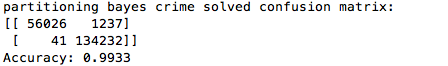
\includegraphics[width=0.5\linewidth]{../Images/PartitioningNaiveBayesCM}
  \caption{Naive Bayes confusion matrix using partitioning}
  \label{fig:PNBCM}
\end{figure}

Even if we tried to change the training and test set, the results were almost identical, so we knew that this kind of accuracy was likely due to some error in the process. Just to be sure, we tried to see if the results changed significantly with cross validation, as can be seen in figure \ref{fig:CVNBCM}, but to no avail.

\begin{figure}[h]
  \centering
  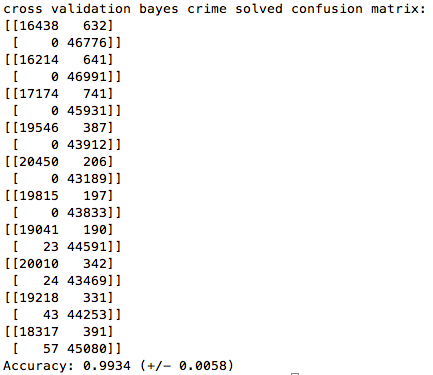
\includegraphics[width=0.5\linewidth]{../Images/CVNaiveBayesCM}
  \caption{Naive Bayes 10-CV confusion matrices-}
  \label{fig:CVNBCM}
\end{figure}

\subsection{Decision Tree}

After the results given by the Naive Bayes predictor, we were really interested to see if and what variables were causing this anomaly. We thought a decision tree could give us that information, and also it seemed like it would be a good fit for the problem. As before, we configured the classifier to predict if a crime was solved or not. The results of the cross validation were similar to Naive Bayes, as seen in figure \ref{fig:PDTCM}.

\begin{figure}[h]
  \centering
  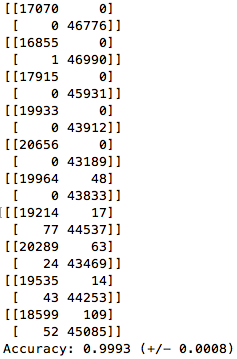
\includegraphics[width=0.25\linewidth]{../Images/PerfectDecisionTreeCM}
  \caption{First Decision tree 10-CV confusion matrices}
  \label{fig:PDTCM}
\end{figure}


So afterwards we proceeded to look at the construction of our predictor. The variables that were used in the high levels o the tree proved very helpful to determine the cause of such high accurate scores, as we can see in figure \ref{fig:PDT}.

\begin{figure}[h]
  \centering
  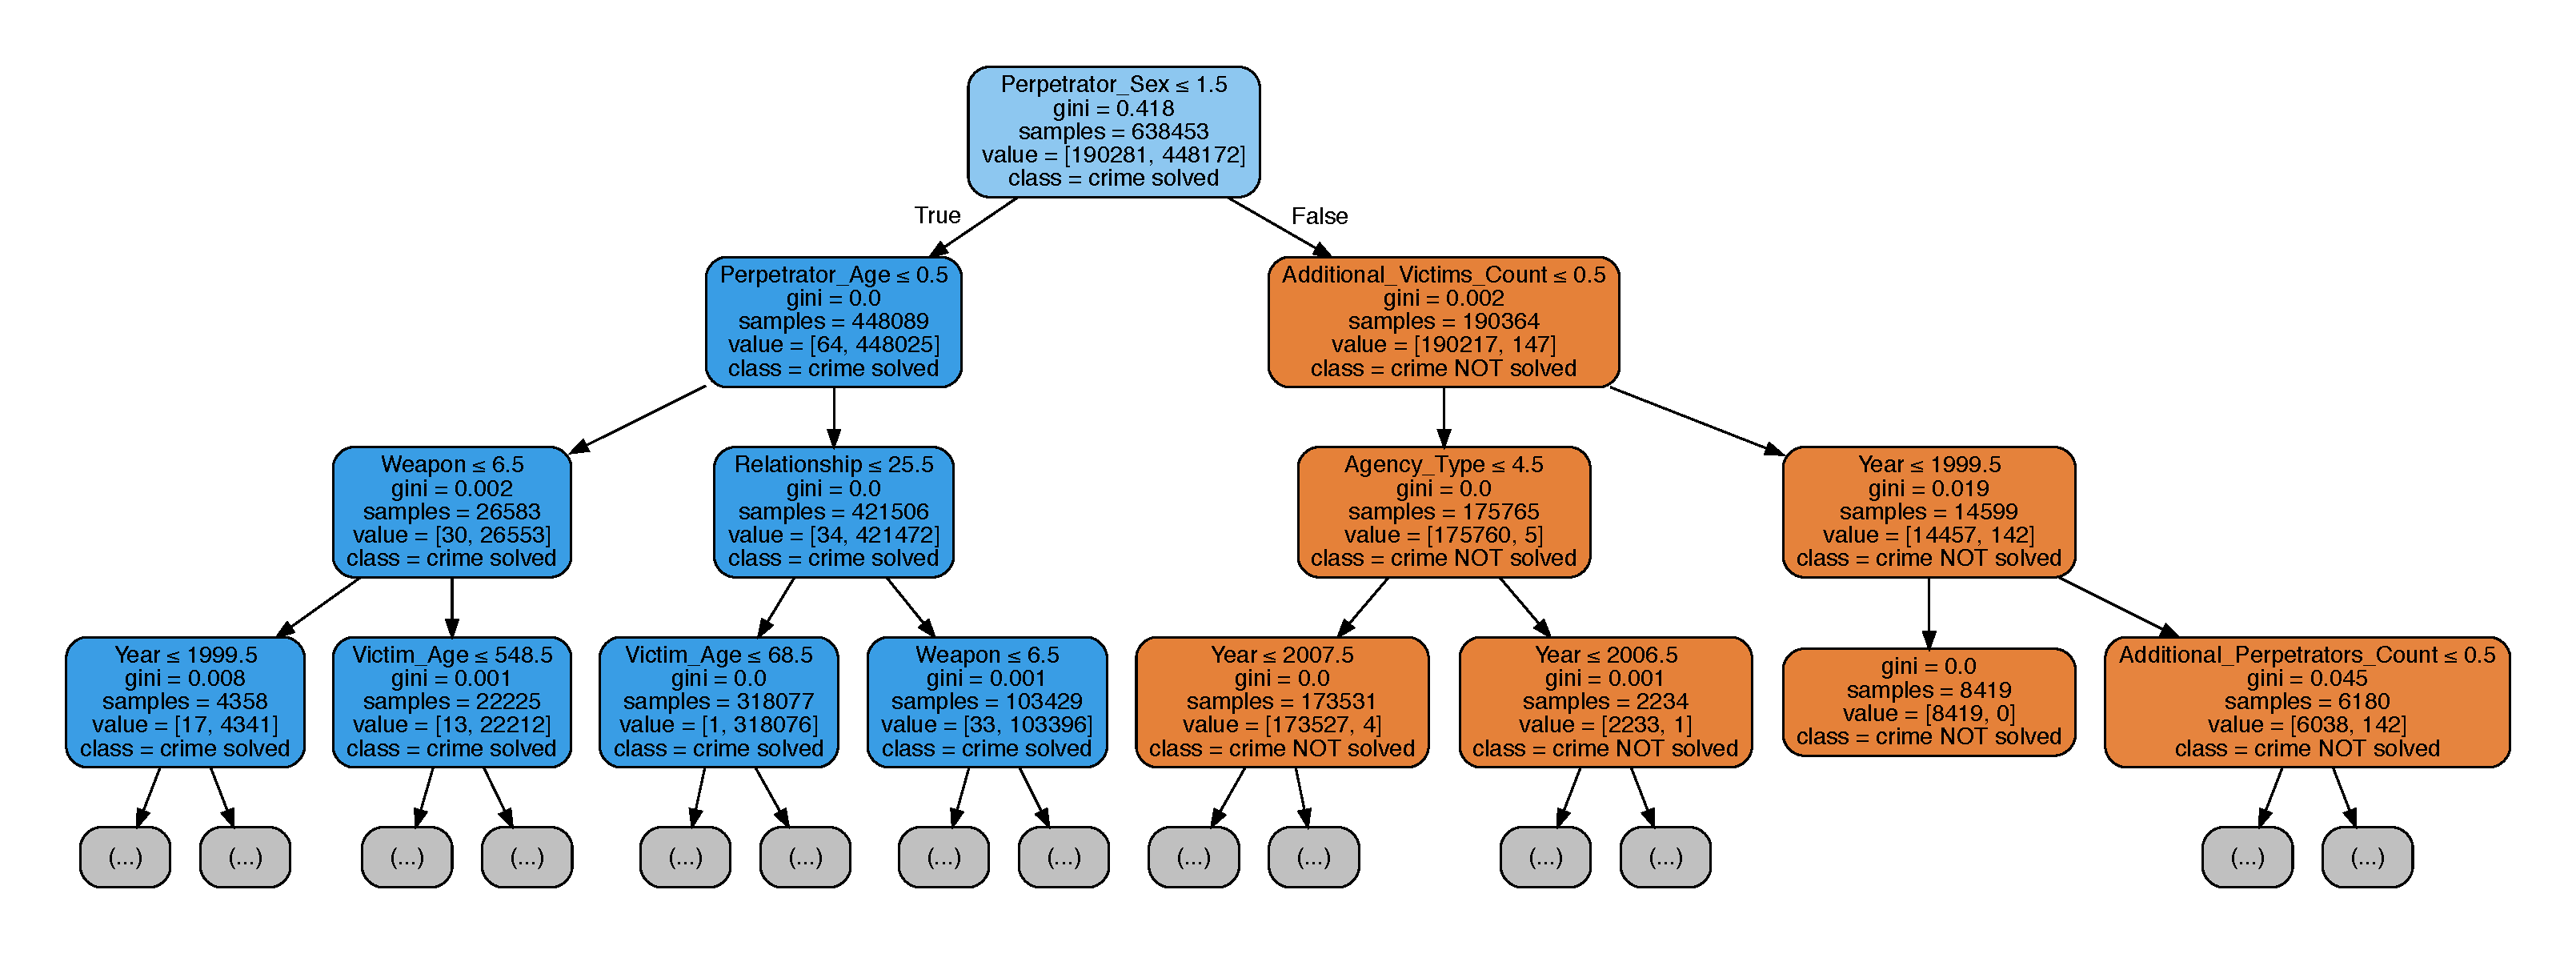
\includegraphics[width=\linewidth]{../Images/PerfectDecisionTree}
  \caption{First Decision tree}
  \label{fig:PDT}
\end{figure}

As we can see, the main way to distinguish between a crime solved and a crime not solved is to see what is the sex of the perpetrator. If the sex is unknown(value 2), then the crime is almost always not solved! But this is obvious, so we don't want to consider this variable to predict if a crime is solved or not. In the same fashion, the perpetrator age can classify if a crime has been solved too accurately.
We then got rid of all variables that describes the perpetrator and his/her relationship to the victim, and proceeded to classify the tree again. The results were much different this time, as seen in figures \ref{fig:RDTCM} and \ref{fig:RDT}.

\begin{figure}[h]
  \centering
  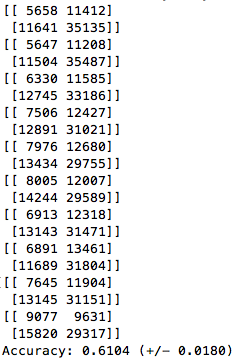
\includegraphics[width=0.25\linewidth]{../Images/RealDecisionTreeCM}
  \caption{Second Decision tree 10-CV confusion matrices}
  \label{fig:RDTCM}
\end{figure}

\begin{figure}[h]
  \centering
  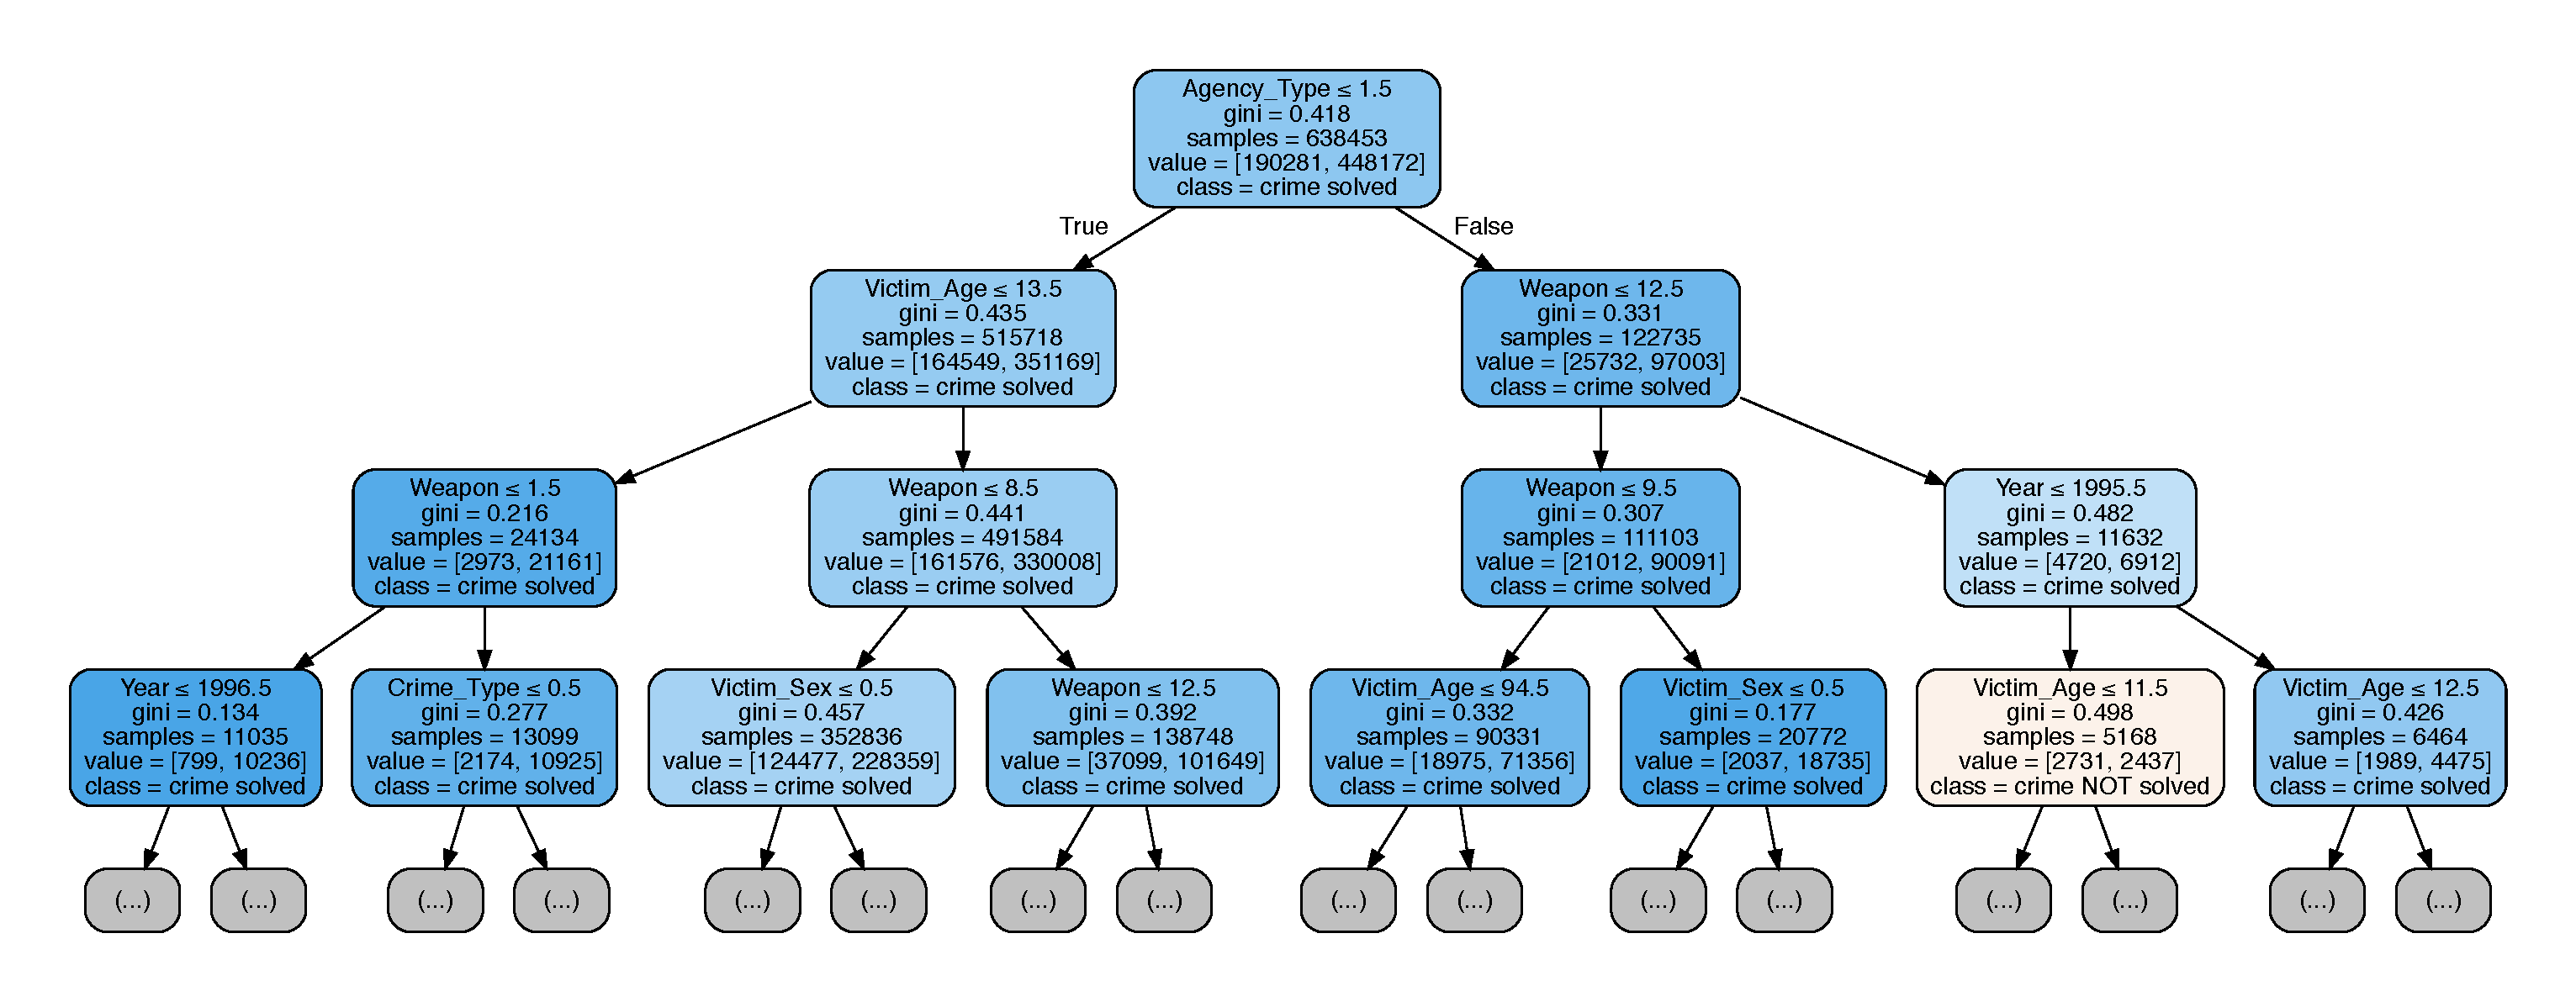
\includegraphics[width=\linewidth]{../Images/RealDecisionTree}
  \caption{Second Decision tree}
  \label{fig:RDT}
\end{figure}

As we can see, the classification is much worse, but seems like a legit one. We can observe the main ways to know beforehand if a crime is hard to solve:
\begin{enumerate}
\item The county or the municipal police are the police department that investigates the case. This is logical, as a smaller police department will have less means to catch the culprit (and also specialized departments are only called when they know they will perform better than more common means.
\item The weapon is not known. This is fairly straightforward, as knowing the weapon used in the crime leads to key clues to solve it.
\item The year of the crime is older or equal to 1995. This is also logical, as technology evolves very rapidly nowadays, and new crucial techniques for investigation become available in a matter of years.
\end{enumerate}

So, even if the classification has only an accuracy of approximately 60 percent, we managed to understand the key characteristics of tackling the problem of solving a crime which is what we were looking for.

\subsection{K-Nearest Neighbours (KNN)}

\subsection{Predictor Application}

\section{Final Thoughts} 
After trying out this library we have reached some mixed feelings about it:
\begin{itemize}
\item[+] It provides a very deep way of implementing machine learning, that is to say that the functions included on this library are very specific in their function, and you are free to implement your own way of doing stuff.
\item[+] Being in python mean that it may be one of the best ways to intertwine both algorithm programming and machine learning easily.
\item[-] It's not that clear what is happening on each step, even when using python IDEs or printing outputs, you hardly get a clear idea of the process that your data goes through, or what's the state of it at each step.
\item[-] The documentation is confusing at times, and relatively not that many people uses this library.
\item[-] The classes included could use more functions at times, and this functions would also improve if they could adapt to different inputs and outputs (for example, needing that all variables to be numerical, and not doing the conversion internally).
\end{itemize}

In conclusion, we think we would use this library only when we already had a clear idea of the data and a specific objective in mind. Also it can be useful if you need to implement advanced algorithms alongside your machine learning code.

Nevertheless, to get a first idea of the data, and in most cases in general, Knime seems to be much more useful and fast, or if we needed something more specific R should provide a more clear way to implement machine learning.

In respect to the database itself, it seemed like a very fun database to play with, having a lot of different ways you can test different techniques. Also the conclusions we reached on each of the sections were very interesting.


\end{document}


%\begin{figure}[h]
%  \centering
%  \includegraphics[width=.5\linewidth]{NB}
%  \caption{Naive Bayes Results}
%  \label{fig:NB}
%\end{figure}

%\begin{figure}[h]
%  \centering
%  \includegraphics[scale=0.5]{decision_tree_partition_confusion_matrix}
%  \caption{Confusion matrix of the decision tree using partition(70\% training, 30\% test)}
%  \label{fig:CMPDT}
%\end{figure}

%-------------------------------------------------------------------------------
% SNIPPETS
%-------------------------------------------------------------------------------

%\begin{figure}[!ht]
%	\centering
%	\includegraphics[width=0.8\textwidth]{file_name}
%	\caption{}
%	\centering
%	\label{label:file_name}
%\end{figure}

%\begin{figure}[!ht]
%	\centering
%	\includegraphics[width=0.8\textwidth]{graph}
%	\caption{Blood pressure ranges and associated level of hypertension (American Heart Association, 2013).}
%	\centering
%	\label{label:graph}
%\end{figure}

%\begin{wrapfigure}{r}{0.30\textwidth}
%	\vspace{-40pt}
%	\begin{center}
%		\includegraphics[width=0.29\textwidth]{file_name}
%	\end{center}
%	\vspace{-20pt}
%	\caption{}
%	\label{label:file_name}
%\end{wrapfigure}

%\begin{wrapfigure}{r}{0.45\textwidth}
%	\begin{center}
%		\includegraphics[width=0.29\textwidth]{manometer}
%	\end{center}
%	\caption{Aneroid sphygmomanometer with stethoscope (Medicalexpo, 2012).}
%	\label{label:manometer}
%\end{wrapfigure}

%\begin{table}[!ht]\footnotesize
%	\centering
%	\begin{tabular}{cccccc}
%	\toprule
%	\multicolumn{2}{c} {Pearson's correlation test} & \multicolumn{4}{c} {Independent t-test} \\
%	\midrule	
%	\multicolumn{2}{c} {Gender} & \multicolumn{2}{c} {Activity level} & \multicolumn{2}{c} {Gender} \\
%	\midrule
%	Males & Females & 1st level & 6th level & Males & Females \\
%	\midrule
%	\multicolumn{2}{c} {BMI vs. SP} & \multicolumn{2}{c} {Systolic pressure} & \multicolumn{2}{c} {Systolic Pressure} \\
%	\multicolumn{2}{c} {BMI vs. DP} & \multicolumn{2}{c} {Diastolic pressure} & \multicolumn{2}{c} {Diastolic pressure} \\
%	\multicolumn{2}{c} {BMI vs. MAP} & \multicolumn{2}{c} {MAP} & \multicolumn{2}{c} {MAP} \\
%	\multicolumn{2}{c} {W:H ratio vs. SP} & \multicolumn{2}{c} {BMI} & \multicolumn{2}{c} {BMI} \\
%	\multicolumn{2}{c} {W:H ratio vs. DP} & \multicolumn{2}{c} {W:H ratio} & \multicolumn{2}{c} {W:H ratio} \\
%	\multicolumn{2}{c} {W:H ratio vs. MAP} & \multicolumn{2}{c} {\% Body fat} & \multicolumn{2}{c} {\% Body fat} \\
%	\multicolumn{2}{c} {} & \multicolumn{2}{c} {Height} & \multicolumn{2}{c} {Height} \\
%	\multicolumn{2}{c} {} & \multicolumn{2}{c} {Weight} & \multicolumn{2}{c} {Weight} \\
%	\multicolumn{2}{c} {} & \multicolumn{2}{c} {Heart rate} & \multicolumn{2}{c} {Heart rate} \\
%	\bottomrule
%	\end{tabular}
%	\caption{Parameters that were analysed and related statistical test performed for current study. BMI - body mass index; SP - systolic pressure; DP - diastolic pressure; MAP - mean arterial pressure; W:H ratio - waist to hip ratio.}
%	\label{label:tests}
%\end{table}